\chapter{研究の背景}
\label{chap:background}

本章ではまず提案手法の核となる技術であるDVFS、及びDVFSを用いた既存の電力削減手法について説明する。そして、対象とする蓄電池を含んだシステムの電力供給システムについて説明した後、蓄電池とDVFSの両方を用いた電力削減手法の関連研究を紹介する。

\section{DVFS}
\label{sec:dvfs}

\subsection{DVFSとは}
プロセッサやメモリを省電力化する最も単純な手法の一つとして、DVFS(Dynamic Voltage and Frequency Scaling)というものがある。
これは、プロセッサやメモリの動作周波数を、負荷状況に応じて動的に変更するというものである。
ただし、動作周波数が高いほど処理能力も高くなるが、同様に消費電力も大きくなる。
かつてプロセッサやメモリは設計時に決められた一つの動作周波数でしか動作することはできなかった。
しかし、省電力化の要求が高まってきたため、現在では一つのプロセッサやメモリが複数の動作周波数をサポートしており、
負荷状況に応じて適切に動作周波数を選択している。


図\ref{fig:dvfs_background}に、あるサーバプロセッサにおける計算負荷(Compute load)と消費電力の関係を動作周波数ごとに示す\cite{Hennessy:2011:CAF:1999263}。横軸は計算負荷を、縦軸は消費電力を示している。動作周波数を低くすることにより処理できる最大負荷は下がるが、電力を削減することもできている。つまり、処理できる負荷であれば低い動作周波数の方が消費電力を少なくすることができる。図\ref{fig:dvfs_background}で1GHzの場合と2.4GHzの場合を比較すると、動作周波数を下げることにより最大で20\%ほどの電力削減が行えることになる。

\begin{figure}[t]
 \begin{center}
  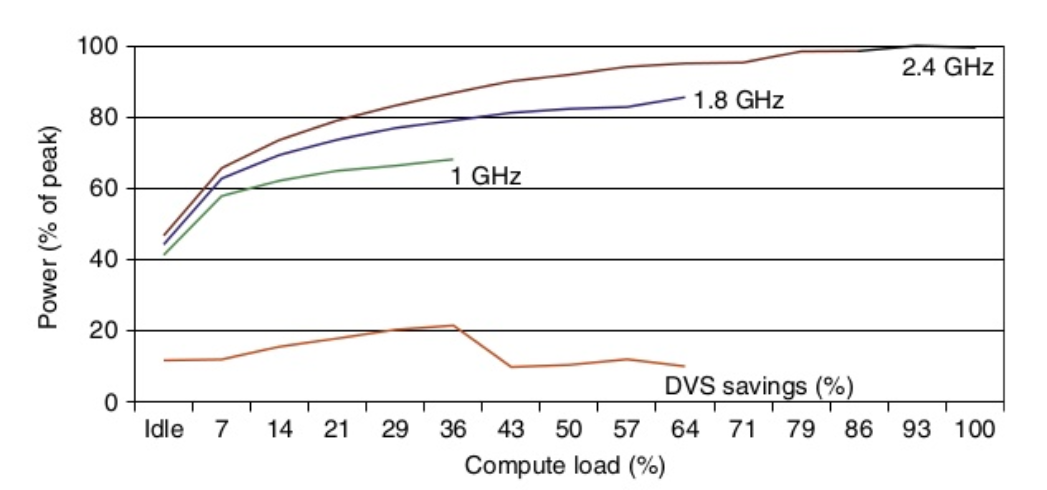
\includegraphics[width=110mm]{DVFS_background.png}
 \end{center}
 \caption{DVFSによる電力削減(AMD Opetron microprocessor) 文献\cite{Hennessy:2011:CAF:1999263} Figure 1.12より}
 \label{fig:dvfs_background}
\end{figure}



\subsection{DVFSを用いたコンピュータの既存の省電力化手法}
これまで、DVFSに関する研究は多く行われてきた。本節ではこれら既存研究や、
具体的なDVFSの利用シナリオの例について述べる。


プロセッサに対してDVFSを適用する研究はこれまでに多くなされており、
現行のプロセッサにも実装される程普及している。
特に、近年では主流となっている1チップ上に複数のコアを搭載したCMP(Chip Multiprocessor)上では効果的である。
例えば、CMP上で並列アプリケーションを実行した場合、同期待ちによって処理を行わないコアが生じる。
そのような状況では、処理を行っているひとつのコアのみを高い周波数で動作させ、
その他のプロセッサの動作周波数を落とす手法が有効である。
さらに、文献\cite{4658633}では、複数プロセッサの組み込みシステムにおいて、
ナノ秒単位でDVFS制御を行うことにより既存のDVFS制御からさらに20\%もの電力削減が行えるとされている。


また、メモリに対するDVFSについても、近年いくつかの研究がなされている。
例えば、文献\cite{David:2011:MPM:1998582.1998590}では、
メモリのバンド幅の使用率を用いてメモリのDVFS制御を行うことによ
り、システム全体のエネルギーの2.4\%を削減できることが示されている。
さらに、文献\cite{6493615}ではプロセッサとメモリのDVFSを同時に用いることによって、
それぞれのDVFSを別々に行う場合よりもさらに電力あたりの性能の向上を目指している。
この手法では、5ミリ秒おきにプロセッサとメモリの処理能力の両方を監視して、一方のモジュールの処理能力が足りないときにはそのモジュールに電力を融通することによって処理能力の偏りをなくし、与えられた性能制約を満たしつつ省電力化を行っている。

HPC(High Performance Conputing)領域においてもDVFSを用いて、消費電力に対する性能を高めようと研究も多く行われている\cite{Rountree:2009:AMD:1542275.1542340}。HPCでは処理能力が高いことが強く求められるため、省電力化を行う場合でも、性能低下ができる限り小さくなるような手法を確立することが強く要求されている。

%プログラム実行時、メモリやネットワークなどのプロセッサ以外のモジュールがボトルネックとなっているときには、プロセッサは処理を行わず電力だけを消費している時間の割合が高くなる。
%そのためこのような状況ではプロセッサ自体の処理能力を落としてもシステム全体の処理能力はあまり下がらないため、

%プロセッサを低い動作周波数に切り替えることで性能低下を防ぎつつ省電力化を行ってきた。




%以上はプロセッサまたはメモリのDVFSをそれぞれ個別に行う手法であったが、プロセッサとメモリのDVFSを協調して行うことにより、さらなる性能向上を目指す手法も存在する。一般に、プログラム実行時はプロセッサかメモリのどちらかの処理能力がシステム全体のボトルネックとなっていることが多く、このときボトルネックとなっていないモジュールでは処理能力が必要以上に高い状態となっており、電力が無駄に消費されている。そのため、それぞれのモジュール間での処理能力の差をなくすことが、無駄な電力消費を減らす上で重要である。

%この問題を解決するため、



\section{蓄電池を含む電力供給システム}
\label{sec:ups}

スーパーコンピュータやデータセンタなどの大規模高性能計算システムにおいては、高い信頼性や可用性が要求されるため、一瞬たりとも電圧低下や電力供給停止は許されない。そのため、停電や機器の故障によって電力会社からの電力供給が受けられない時にも、コンピュータへの電力供給を継続するためにいくつかの冗長電源設備が用意されている。図\ref{fig:power_distribution_background}は本論文で対象とする高性能計算システムの電源設備である。
\begin{figure}[t]
 \begin{center}
  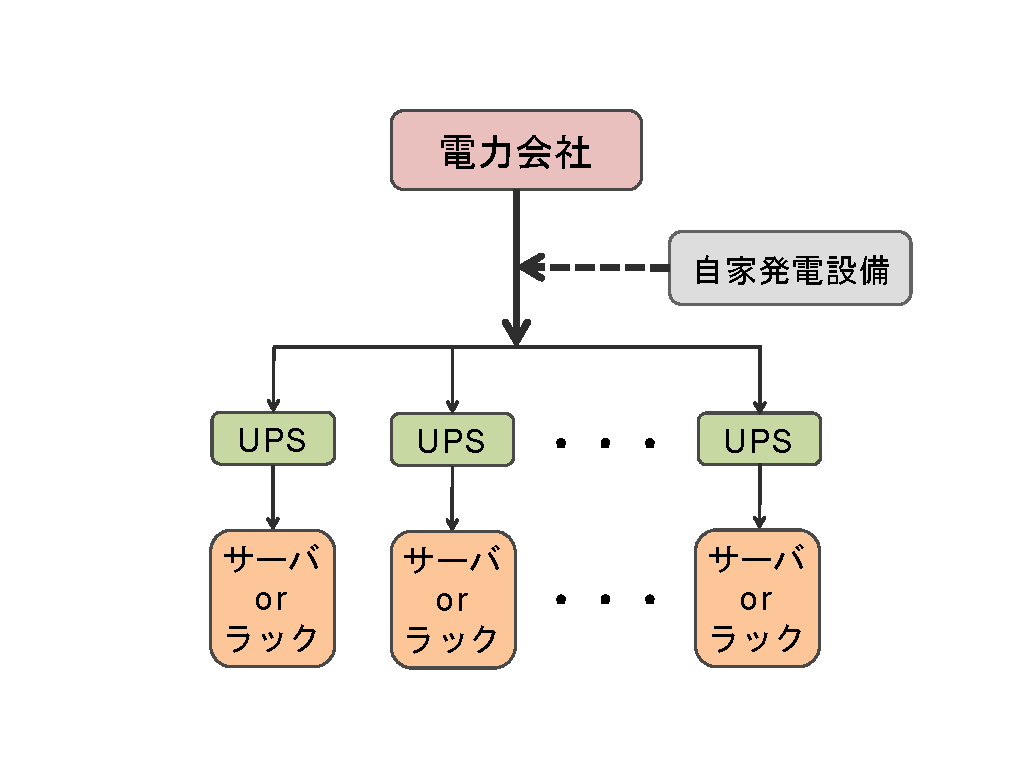
\includegraphics[width=120mm]{power_distribution_background.eps}
 \end{center}
 \caption{本論文で対象とする高性能計算システムの電源設備}
 \label{fig:power_distribution_background}
\end{figure}

一般的な高性能計算システムでは、システム全体にひとつのUPS(無停電電源装置)が搭載されているが、GoogleやFacebookのデータセンタにおいては図\ref{fig:power_distribution_background}一つのラックやサーバごとにUPSが搭載されている\cite{Datacenter}。これは電力架線からサーバまでの電力供給の間に行われるD/A変換の回数を減らして、全体での電力変換効率を向上させるためである。このように、ラックごとやサーバごとなどの細かい単位でのUPSを配置する方法は、電力効率を重視する上ではこれからのスタンダードになっていくと考えられている。

UPSを搭載したデータセンタにおいて電力会社からの電力供給が停止した場合には、UPSが電力供給を行い、同時に自家発電設備が起動する。数分後、自家発電設備が完全に起動して電力供給が可能になると、自家発電設備から電力供給が行われるようになる。電力会社からの電力供給が再開すると自家発電設備は停止し、電力会社からの電力を使用するようになる。

ここでUPSは3つの役割を担っている。一つ目は、コンピュータへの供給電圧を安定させること。二つ目は、停電時に自家発電設備からの電力供給が始まるまでの間、電力を供給すること。三つ目は、停電復帰後に自家発電設備から電力会社に電力供給元を切り替えるとき、一時的に電力供給を行うことである。

UPS単体がシステム全体に電力を供給し続けられる時間は数分〜30分程度である場合が多い。現在の多くのUPSでは電源として蓄電池が使用されているが、充放電が行われるのは基本的に停電時のみであり、今のところ平常時に積極的に充放電を行うような使い方はなされていない。



\section{データセンタにおける蓄電池を用いたピーク電力削減手法}
\label{sec:capping}

前\ref{sec:ups}節で述べたように、今までは平常時に積極的にUPSの蓄電池から充放電を行うことはなかったが、2011年に発表された論文\cite{Govindan:2011:BLT:2024723.2000105}において、UPSからの充放電を用いたデータセンタの電力ピークカット手法が提案された。本稿の提案手法と大きく関わる内容であるので、ここで詳しく紹介する。

データセンタにおいてはコンピュータでの消費電力や冷却にかかる電力コストは全体の運用コストの10〜30\%に上り、サービス向上のために電力コストの削減が必要とされている。データセンタを建設するときの初期投資、及び電力会社との契約料金はピーク時の電力に大きく影響される。そのためピーク電力を削減すべく、この論文ではUPSの中の蓄電池を用いた電力ピークカット手法を提案している。

データセンタの1日の電力需要の推移は、統計や過去の研究によってある程度予測ができるようになっている。その電力需要曲線から最適な蓄電池の充放電計画を立て、電力会社から引き込む電力の最大値を低く抑えることがこの紹介論文の主旨である(図\ref{fig:power_graph_datacenter})。
\begin{figure}[t]
 \begin{center}
  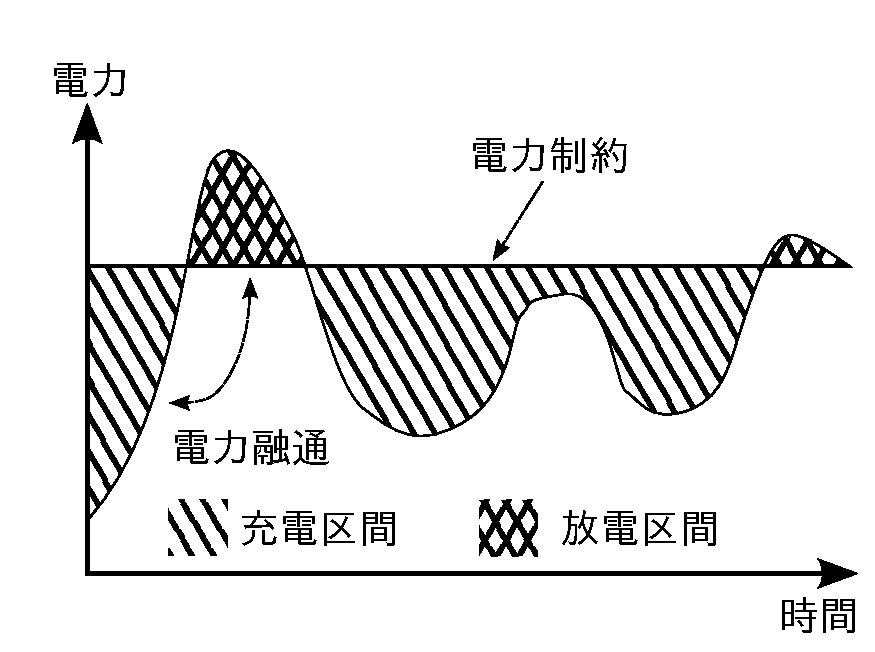
\includegraphics[width=90mm]{power_graph_datacenter.eps}
 \end{center}
 \caption{参考文献\cite{Govindan:2011:BLT:2024723.2000105}における蓄電池を用いた電力ピークカット手法}
 \label{fig:power_graph_datacenter}
\end{figure}

紹介論文において解くべき対象としている問題を言葉で表現すると以下のようにまとめられる。

\begin{itemize}
  \item 目的
    \begin{itemize}
      \item minimize (一日の最大消費電力)
    \end{itemize}
  \item 与えられる情報
    \begin{itemize}
      \item 一日の電力推移グラフ
    \end{itemize}
  \item 制御対象
    \begin{itemize}
      \item バッテリーをいつ、どれだけ充放電するか
    \end{itemize}
  \item 制約条件
    \begin{itemize}
      \item 一日の放電時間・回数
      \item バッテリーの残量
    \end{itemize}
\end{itemize}

この紹介論文の研究以前にも、電力会社からのピーク電力を削減するためにプロセッサの動作速度を変更する手法\cite{Chen:2005:MSE:1064212.1064253,Isci:2006:AEM:1194816.1194850,Raghavendra:2008:NPS:1353534.1346289,4658632,4658631}や、負荷を時間的もしくは空間的に分散させる手法\cite{Unleash,Moore:2005:MSC:1247360.1247365}が提案されてきた。しかし、これらの手法を適用すると処理速度の低下が必ず起こってしまうことが問題であった。紹介論文における提案手法は、UPSに含まれるバッテリーという既存設備を用いることで、この性能低下を起こさずに電力ピークカットを実現できることを示している。

この手法で実際に用いられているアルゴリズムは図で表現すると図\ref{fig:algo}のようになり、言葉で表現すると以下のようになる。

\begin{enumerate}
  \item 一番高いピークが、二番目に高いピークと同じ高さになるように放電を計画(制約条件を満たせば次のステップへ)
  \item 二番目のピークより高いピーク全てが、三番目に高いピークと同じ高さになるように放電を計画(制約条件を満たせば次のステップへ)
  \item ・・・(制約条件を満たさなくなるまで繰り返し)
\end{enumerate}

\begin{figure}[t]
 \begin{center}
  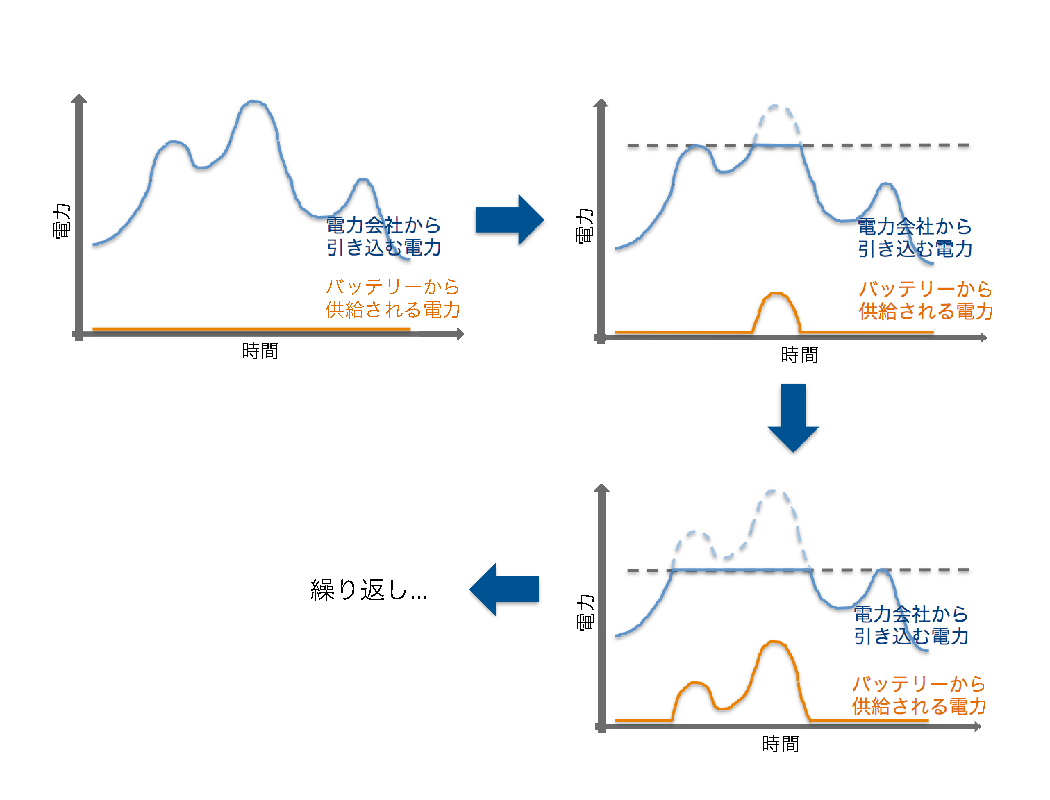
\includegraphics[width=140mm]{algo.eps}
 \end{center}
 \caption{紹介論文\cite{Govindan:2011:BLT:2024723.2000105}におけるUPSを用いた電力ピークカットアルゴリズム}
 \label{fig:algo}
\end{figure}

この紹介論文は他にもバッテリーの電力を使用することによる停電時の信頼性低下や、充放電頻度に対するバッテリーの寿命低下も考慮に入れて充放電計画を立てることによって、データセンタの事業継続性を保ちつつ電力コストを削減できるとしている。

この紹介論文では性能制約を守った上でどれだけ省電力化を行えるのかという問題であった。一方で、決められた電力制約を超えないように制御を行うPower Cappingという手法についての先行研究も存在する\cite{Fan:2007:PPW:1273440.1250665}。Power Cappingを実現するためには様々なアプローチがあるが、定期的に使用電力を監視して電力制約に近づくとプロセッサの周波数を下げる・実行するタスクを減らす、といったような手法が提案されている。




